\section{Nanoservices}
\label{sec:nanoservices}
Nanoservices are a new framework for building compute-intensive, distributed applications with the following three characteristics:

\vspace{0.5pt}
\begin{itemize}
    \item[\bf C1:] Each application is divisible into compute-intensive {\em nanotasks}.
    \item[\bf C2:] Each nanotask is able to process and respond to network messages in under \SI{1}{\mu s}.
    \item[\bf C3:] The working set of each nanotask fits in the L1 cache.\footnote{L1 cache is typically \SI{256}{kB}--\SI{1}{MB} at the time of writing, including the data and instruction cache.}
\end{itemize}
\vspace{0.5pt}

Figure~\ref{fig:app-frameworks} highlights the key differences between nanoservices and two other major application development frameworks: monoliths and microservices.
We believe that many applications can benefit from the nanoservices framework, including applications such as physical simulations~\cite{barnes-hut, molecular-dynamics}, neural-network inference and training~\cite{tensorflow}, graphics processing~\cite{ray-tracing}, and state-space search algorithms~\cite{state-space-search}.
As we will show in \S\ref{sec:evaluation}, total application runtime has the potential to be reduced by about three orders of magnitude if they are implemented using nanoservices.

The central idea is as follows: A nanotask must execute in the shortest, and most deterministic time possible. 
This implies that {\em everything} the nanotask needs must sit in registers and the L1 cache: Instructions in the L1 instruction cache, and data (in-progress messages, variables and program state) in registers or the L1 data cache. 
Cache misses are expensive, and the goal is to avoid them--L2 cache and external memory are, respectively, ten and one hundred times slower than the L1 cache~\cite{jeff-dean-numbers}.

Building nanoservices requires more than simply dividing applications into nanotasks that access small amounts of data.
We also need to consider how to quickly and predictably transfer message data between the wire and an application thread, and how to efficiently schedule nanotasks on the available processor cores.
It is not practical to run nanoservices on today's systems, which were designed to support applications that process RPCs in milliseconds, or at best tens of microseconds~\cite{eRPC, perfkit-grpc}, not hundreds of nanoseconds.
Addressing these problems therefore requires hardware changes, which we address with our proposed design, the \name{}, in the following section.

\begin{figure}
  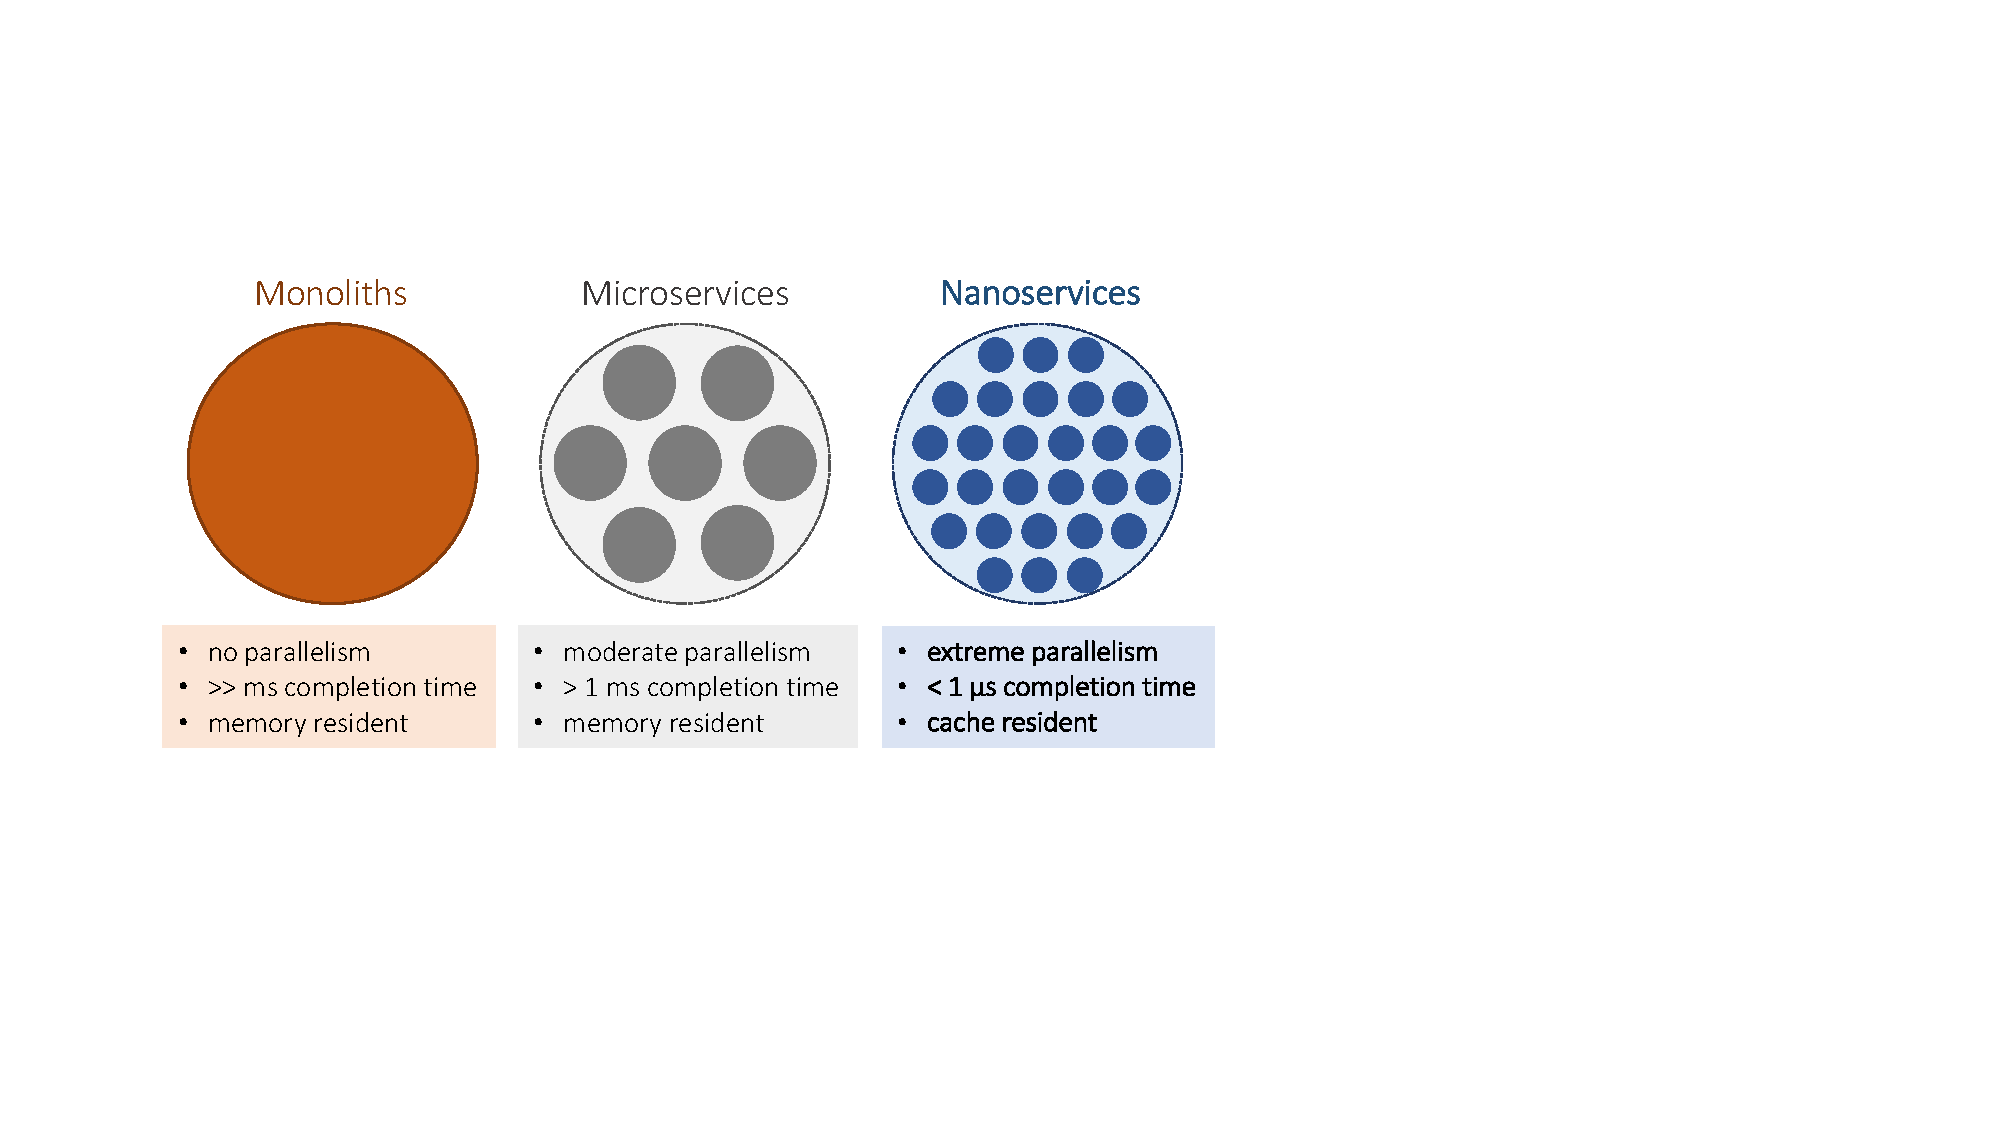
\includegraphics[width=0.9\linewidth]{./figures/app-frameworks}
  \caption{A comparison of key characteristics of {\em nanoservices} vs. monoliths and microservices.}
  \label{fig:app-frameworks}
\end{figure}
